% Nejprve uvedeme tridu dokumentu s volbami
\documentclass[czech,master,dept460,male,cpp,cpdeclaration]{diploma}
\usepackage{graphicx}
\graphicspath{ {./images/} }
% Dalsi doplnujici baliky maker
\usepackage[autostyle=true,czech=quotes]{csquotes} % korektni sazba uvozovek, podpora pro balik biblatex
\usepackage[backend=biber, style=iso-numeric, alldates=iso]{biblatex} % bibliografie
\usepackage{dcolumn} % sloupce tabulky s ciselnymi hodnotami
\usepackage{subfig} % makra pro "podobrazky" a "podtabulky"

% Zadame pozadovane vstupy pro generovani titulnich stran.
\ThesisAuthor{Jakub Pšenčík}

\CzechThesisTitle{Podpora jazyka Monkey C v prostředí VS Code}

\EnglishThesisTitle{Monkey C Language Support in VS Code}

\SubmissionDate{1. září 2020}

% Pokud nechceme nikomu dekovat makro zapoznamkujeme.
\Thanks{Rád bych na tomto místě poděkoval svému vedoucímu práce Ing. Janu Janouškovi za odborné a metodické vedení, ochotu a pomoc v průběhu vypracovávání práce.}

% Zadame cestu a jmeno souboru ci nekolika souboru s digitalizovanou podobou zadani prace.
% Pokud toto makro zapoznamkujeme sazi se stranka s upozornenim.
\ThesisAssignmentImagePath{Figures/Assignment}



% Zadame soubor s digitalizovanou podobou prohlaseni autora zaverecne prace.
% Pokud toto makro zapoznamkujeme sazi se cisty text prohlaseni.
%\AuthorDeclarationImageFile{Figures/AuthorDeclaration.jpg}


% Zadame soubor s digitalizovanou podobou souhlasu spolupracujici prav. nebo fyz. osoby.
% Pokud toto makro zapoznamkujeme sazi se cisty text souhlasu.
%\CooperatingPersonsDeclarationImageFile{Figures/CoopPersonDeclaration.jpg}

\CzechAbstract{V této bakalářské práci se budu zabývat vývojem rozšíření pro Visual Studio Code, jenž bude poskytovat plnou podporu jazyka Monkey C. Součástí práce bude bude představení prostředí Visual Studio Code a problematika vývoje rozšíření v tomto prostředí. Představen bude, mimo jiné, také jazyk Monkey C. V další části práce se budu zabývat nástrojem ANTLR, díky kterému jsme schopni generovat vlastní překladač jazyka pomocí bezkontextové gramatiky, parsováním kódu a jeho syntaktickou analýzou. Závěrem bude výsledné rozšíření testováno.}

\CzechKeywords{bakalářská práce, rozšíření, Monkey C, Typescript}

\EnglishAbstract{In this bachelor thesis I will deal with the development of extension for Visual Studio Code, which will provide full support for Monkey C language. The work will include an introduction to the Visual Studio Code environment and the development of extensions in this environment. Among other things, the Monkey C language will be introduced. In the next part of the work I will describe the ANTLR tool, used to generate our own language compiler using context-free grammar, code parsing and its syntactic analysis. Finally, the resulting extension will be tested.}

\EnglishKeywords{bachelor thesis, extension, Monkey C, Typescript}

\AddAcronym{ANTLR}{ANother Tool for Language Recognition}



\addbibresource{biblatex-examples.bib}

% Novy druh tabulkoveho sloupce, ve kterem jsou cisla zarovnana podle desetinne carky
\newcolumntype{d}[1]{D{,}{,}{#1}}


% Zacatek dokumentu
\begin{document}

% Nechame vysazet titulni strany.
\MakeTitlePages
% A nasleduje text zaverecne prace.
\section{Úvod}
\label{sec:Introduction}
Tato bakalářská práce se věnuje tvorbě a vývoji rozšíření pro vývojové prostředí Visual Studio Code. Cílem práce je vytvořit takové rozšíření, která poskytne plnou podporu při vývoji aplikací v jazyce Monkey C. Jedná se o dynamicky postavený jazyk, stejně jako např. python, R, atd… Jazyk se používá k vývoji aplikací pro Garmin zařízení.\\ V další kapitolách budou detailně popsány klíčové komponenty k vytvoření finální aplikace, např. gramatika pro popis jazyka, ANTLR parser, atd... 



\section{Problematika vývoje rozšíření pro VS Code}
\subsection{Visual Studio Code}
Visual Studio Code je editor zdrojového kódu vytvořený společností Microsoft pro Windows, Linux a MacOS. Nabízí spoustu užitečných funkcí, mezi které patří podpora ladění kodu, zvýrazňování syntaxe, automatické doplňování a našeptávání kódu, atd…


\subsection{Typescript}
TypeScript$^{[1]}$ je open-source programovací jazyk vyvinutý společností Microsoft. Jedná se o nádstavbu nad jazykem JavaScript,
která jej rozšiřuje o statické typování a další atributy, které známe z objektově orientovaného programování jako jsou třídy, moduly a další. Samotný kód psaný v jazyce TypeScript se kompiluje
do jazyka JavaScript. Jelikož je tento jazyk nádstavbou nad JavaScriptem, je každý JavaScript kód automaticky validním TypeScript kódem.

\subsection{Komponenty potřebné pro vytvoření rozšíření}
Předtím, než začneme pracovat na samotném rozšíření, je potřeba obstarat několik důležitých nastrojů a komponent, jenž jsou klíčové při vývoji.
\subsubsection{Gramatika}
Jako první je potřeba definovat popis jazyka MonkeyC. V našem případě je jazyk popsán prostřednictvím bezkontextové gramatiky, která formálně definuje syntax (pravidla) jazyka.

\begin{center}
	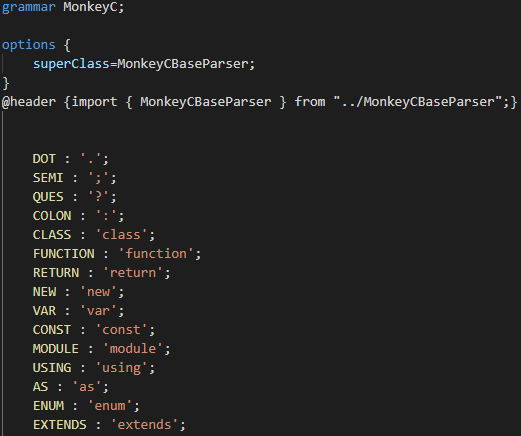
\includegraphics[scale=0.8]{grammar}
	\\
	Obr. 1 – ukázka hlavičky gramatiky MonkeyC.g4 pro popis jazyka
\end{center}

Na obrázku mužeme vidět prvních pár řádků gramatiky pro MonkeyC. Gramatika obsahuje spoustu známých klíčových slov, nebo-li tokenů, např. "CLASS", "FUNCTION", "USING", atd...

\subsubsection{Java}
Jelikož je ANTLR psán v Javě, je potřeba ji nainstalovat na naše zařízení, přičemž se požaduje verze 1.6 nebo vyšší. Poté již stačí stáhnout akualní ANTLR jar, což je momentálně "antlr-4.8-complete.jar".

\subsubsection{Parser a Lexer}
\textbf{lexer} - lexer (nebo také tokinizér) "rozdělí" text na vstupu (v našem případě MonkeyC kód) na tokeny.\\
\textbf{parser} - shora dolů prochází text na vstupu a porovnává jednotlivé řádky s pravidly obsažené v gramatice.\\
K vytvoření parseru a lexeru je potřeba spustit ANLTR nástroj, který s pomocí gramatiky tyto souboru vygeneruje.\\

\begin{center}
	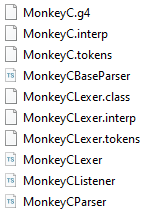
\includegraphics{generated_files}
	\\
	Obr. 2 – potřebné soubory vygenerované nástrojem ANTLR
\end{center}

\subsubsection{TestRig}
ANTLR poskytuje flexibilní testovací nástroj umístněný v runtime knihovně s názvem TestRig. TestRig dokáže poskytnout spoustu informací o tom, jak "recognizéry" (parser a lexer) zpracovávají InputStream ze vstupního souboru.\\
Nejjednodušší způsob ověření, zda gramatika rozpoznává vstup správně, je zobrazit si vygenerovaný syntaktický strom vizuálně.

\begin{center}
	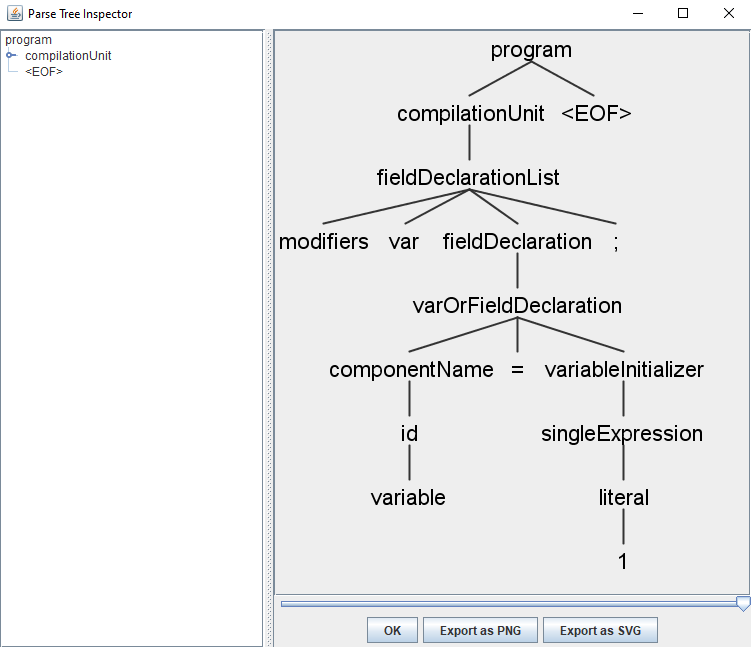
\includegraphics[scale=0.8]{ParseTreeInspector}
	\\
	Obr. 3 – "ParseTreeInspector" - vizuální podoba syntaktického stromu
\end{center}
Na obrázku můžeme detailně vidět jak parser vytvořil syntaktický strom a jak jsou jednotlivé části propojené. Strom začíná kořenem, jenž je v naší gramatice pojmenová, jako "program". Takto je kořen pojmenován při každém parsování. 

\section{Syntaktická a sémantická analýza kódu}
\subsection{ANTLR - Nástroj pro generování překladače}
ANTLR nebo také ANother Tool for Language Recognition (jiný nástroj pro rozpoznávání jazyka)$^{[2]}$ je výkonný nástroj pro generování syntaktických analyzátorů, tzv. "parser". Tento parser je poté schopen číst, zpracovávat, spouštět nebo překládat strukturované textové či binární soubory. Použivá se především k vytváření nových jazyků, nástrojů nebo "frameworků". Využívá bezkontextový jazyk typu LL.
\subsection{LL syntaktický analyzátor}
LL$^{[3]}$ je syntaktický analyzátor shora-dolů pro bezkontextové gramatiky. Analyzuje vstup zleva (Left) doprava a konstruuje nejlevější derivaci (Leftmost) věty. Gramatiky, které jsou takto analyzovatelné, se nazývají LL gramatiky.

\subsection{Syntaktický strom}
Strom, který parser používá např. k detekci syntaktických chyb v kódu
\subsection{Sémantický strom}
Strom, jenž hraje zásadní roli v procesech, jako je našeptávání kódu, detekci chyb, kdy je použita třída z modulu, který není referencován, atd...

\subsection{parser}
Fusce nibh. Sed ut perspiciatis unde omnis iste natus error sit voluptatem accusantium doloremque laudantium, totam rem aperiam, eaque ipsa quae ab illo inventore veritatis et quasi architecto 
beatae vitae dicta sunt explicabo. Quis autem vel eum iure reprehenderit qui in ea voluptate velit esse quam nihil molestiae consequatur, vel illum qui dolorem eum fugiat quo voluptas nulla pariatur? Etiam ligula pede, sagittis quis, interdum ultricies, scelerisque eu. Maecenas sollicitudin. Cras pede libero, dapibus nec, pretium sit amet, tempor quis. Integer vulputate sem a nibh rutrum consequat. Pellentesque sapien. Pellentesque arcu. Suspendisse nisl. Fusce consectetuer risus a nunc. Etiam dui sem, fermentum vitae, sagittis id, malesuada in, quam. Cum sociis natoque penatibus et magnis dis parturient montes, nascetur ridiculus mus. Nam quis nulla. Nulla non lectus sed nisl molestie malesuada. Duis viverra diam non justo. Sed ac dolor sit amet purus malesuada congue. Aenean id metus id velit ullamcorper pulvinar. Aliquam ornare wisi eu metus. Neque porro quisquam est, qui dolorem ipsum quia dolor sit amet, consectetur, adipisci velit, sed quia non numquam eius modi tempora incidunt ut labore et dolore magnam aliquam quaerat voluptatem.


\section{Představení jazyka Monkey C}
Monkey C$^{[4]}$  je objektově orientovaný jazyk navržený pro snadný vývoj Connect IQ aplikací. Jedná se o dynamický programovací jazyk, podobně jako Java, PHP či Ruby. Cílem Monkey C je zjednodušit proces vytváření samotné aplikace a umožnit tak vývojářům více se soustředit na zákazníka a méně na omezení zdrojů. Využívá tzv. "reference counting" k automatickému čištění paměti, což vývojáře osvobozuje od manuální správy paměti (např. jako v jazyce C/C++).
\\
\begin{center}
	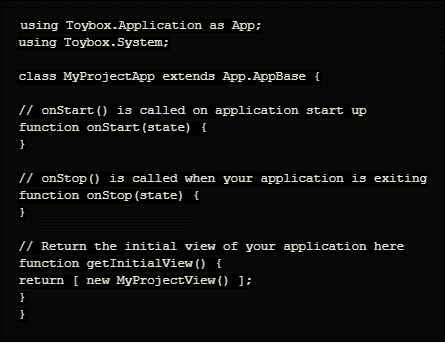
\includegraphics{code_snippet}
	\\
	Obr. 3 – ukázka jednoduchého fragmentu kódu v MonkeyC
\end{center}
	

\section{Návrh a implementace rozšíření pro VS Code}
Rozšíření bude, jak již bylo nastíněno výše, implementováno v jazyce Typescript. 
K vytvoření rozšíření samotného je potřeba Node.js a Git. Poté je vyžadována instalace programu "Yeoman" "VS Code Extension Generator".

\subsection{zvýraznění kódu}

Zvýraznění, nebo-li obarvení klíčových slov kódu je realizováno pomocí JSON souboru, jenž pomocí regulárních výrazů v textu vyhledává příslušná slova a ty poté obarvuje.
\\
\begin{center}
	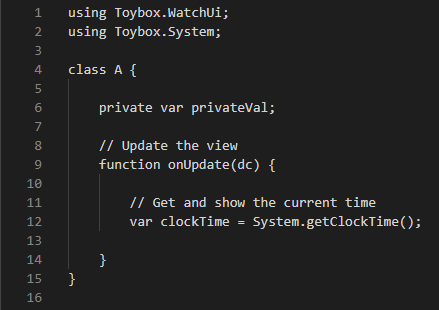
\includegraphics[]{uncolored_code}
	\\
	Obr. 4 – ukázka neobarveného kódu v MonkeyC
\end{center}

\begin{center}

	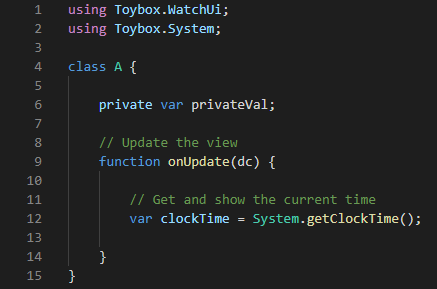
\includegraphics[]{colored_code}
	\\
	Obr. 5 – ukázka obarvení kódu v MonkeyC
\end{center}
	
Hned na první pohled je zřejmé, že obarvení poskytuje uživateli větší přehled a orientaci v kódu, jak je vidět na obrázku [5]


\subsection{Automatické doplňování a našeptávání kódu}

Hlavním aktérem při našeptávání vhodných částí kódu je "antlr4-c3 The ANTLR4 Code Completion Core".

Jedná se o "stroj" sloužící k dokončování gramatického agnostického kódu pro analyzátory založené na ANTLR4. Engine c3 je schopen poskytnout kandidáty na doplnění kódu, kteří jsou užiteční pro editory s analyzátory generovanými ANTLR, nezávisle na skutečném jazyku / gramatice použité pro generování.

Původní implementace je poskytována jako "node module" a je psána v jazyce Typescript.

Pro zobrazení možných symbolů ve zdrojovém kódu zjevně potřebujete zdroj pro všechny dostupné symboly na dané pozici. Jejich poskytnutí je obvykle úkolem tabulky symbolů. Jeho obsah lze odvodit z vašeho aktuálního zdrojového kódu (pomocí analyzátoru + analyzátoru Listeneru). Statičtější části (například runtime funkce) lze načíst z disku nebo poskytnout pevně zakódovaný seznam atd. Tabulka symbolů pak může odpovědět na vaši otázku ohledně všech symbolů daného typu, které jsou viditelné z dané pozice. Pozice obvykle odpovídá konkrétnímu symbolu v tabulce symbolů a struktura pak umožňuje snadno získat viditelné symboly. Engine c3 je dodáván s malou implementací tabulky symbolů, která však není pro použití knihovny povinná, ale poskytuje snadný start, pokud již nemáte vlastní třídu tabulek symbolů.

Zatímco tabulka symbolů poskytuje symboly daného typu, musíme zjistit, který typ je ve skutečnosti vyžadován. To je úkol enginu c3. V nejjednodušším nastavení vrátí pouze klíčová slova (a další symboly lexerů), která jsou povolena gramatikou pro danou pozici (což je samozřejmě stejná pozice, která se používá k nalezení kontextu pro vyhledávání symbolů ve vaší tabulce symbolů). Klíčová slova jsou pevná sada slov (nebo sekvencí slov), která se obvykle nenachází v tabulce symbolů. Skutečné textové řetězce můžete získat přímo ze slovníku analyzátoru. C3 za ně vrací pouze lexerové tokeny.

\begin{center}
	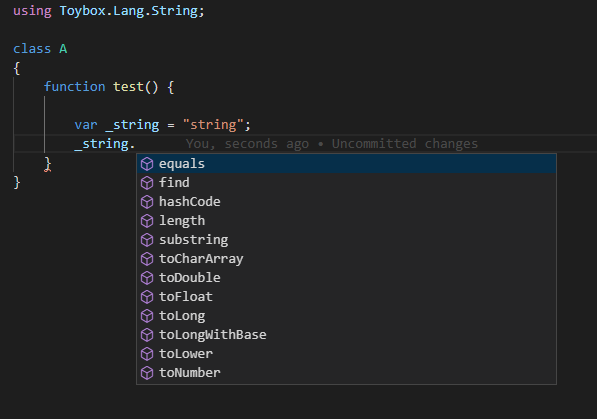
\includegraphics[scale=1]{autocomplete_example}
	\\	
	Obr. 6 – ukázka automatického našeptávání kódu na proměnné typy string
\end{center}


\section{Testování výsledného řešení}
Testování probíhá napříč mnoha fragmenty kódu.


Lorem ipsum dolor sit amet, consectetuer adipiscing elit. Aliquam erat volutpat. Etiam dui sem, fermentum vitae, sagittis id, malesuada in, quam. Donec ipsum massa, ullamcorper in, auctor et, scelerisque sed, est. Vivamus porttitor turpis ac leo. Sed ac dolor sit amet purus malesuada congue. Maecenas aliquet accumsan leo. Etiam posuere lacus quis dolor. Curabitur sagittis hendrerit ante. Duis condimentum augue id magna semper rutrum. Mauris dolor felis, sagittis at, luctus sed, aliquam non, tellus. Integer vulputate sem a nibh rutrum consequat. Duis pulvinar. Duis viverra diam non justo. Aenean vel massa quis mauris vehicula lacinia.

Fusce nibh. Sed ut perspiciatis unde omnis iste natus error sit voluptatem accusantium doloremque laudantium, totam rem aperiam, eaque ipsa quae ab illo inventore veritatis et quasi architecto beatae vitae dicta sunt explicabo. Quis autem vel eum iure reprehenderit qui in ea voluptate velit esse quam nihil molestiae consequatur, vel illum qui dolorem eum fugiat quo voluptas nulla pariatur? Etiam ligula pede, sagittis quis, interdum ultricies, scelerisque eu. Maecenas sollicitudin. Cras pede libero, dapibus nec, pretium sit amet, tempor quis. Integer vulputate sem a nibh rutrum consequat. Pellentesque sapien. Pellentesque arcu. Suspendisse nisl. Fusce consectetuer risus a nunc. Etiam dui sem, fermentum vitae, sagittis id, malesuada in, quam. Cum sociis natoque penatibus et magnis dis parturient montes, nascetur ridiculus mus. Nam quis nulla. Nulla non lectus sed nisl molestie malesuada. Duis viverra diam non justo. Sed ac dolor sit amet purus malesuada congue. Aenean id metus id velit ullamcorper pulvinar. Aliquam ornare wisi eu metus. Neque porro quisquam est, qui dolorem ipsum quia dolor sit amet, consectetur, adipisci velit, sed quia non numquam eius modi tempora incidunt ut labore et dolore magnam aliquam quaerat voluptatem.

\section{Závěr}
Lorem ipsum dolor sit amet, consectetuer adipiscing elit. Aliquam erat volutpat. Etiam dui sem, fermentum vitae, sagittis id, malesuada in, quam. Donec ipsum massa, ullamcorper in, auctor et, scelerisque sed, est. Vivamus porttitor turpis ac leo. Sed ac dolor sit amet purus malesuada congue. Maecenas aliquet accumsan leo. Etiam posuere lacus quis dolor. Curabitur sagittis hendrerit ante. Duis condimentum augue id magna semper rutrum. Mauris dolor felis, sagittis at, luctus sed, aliquam non, tellus. Integer vulputate sem a nibh rutrum consequat. Duis pulvinar. Duis viverra diam non justo. Aenean vel massa quis mauris vehicula lacinia.

Fusce nibh. Sed ut perspiciatis unde omnis iste natus error sit voluptatem accusantium doloremque laudantium, totam rem aperiam, eaque ipsa quae ab illo inventore veritatis et quasi architecto beatae vitae dicta sunt explicabo. Quis autem vel eum iure reprehenderit qui in ea voluptate velit esse quam nihil molestiae consequatur, vel illum qui dolorem eum fugiat quo voluptas nulla pariatur? Etiam ligula pede, sagittis quis, interdum ultricies, scelerisque eu. Maecenas sollicitudin. Cras pede libero, dapibus nec, pretium sit amet, tempor quis. Integer vulputate sem a nibh rutrum consequat. Pellentesque sapien. Pellentesque arcu. Suspendisse nisl. Fusce consectetuer risus a nunc. Etiam dui sem, fermentum vitae, sagittis id, malesuada in, quam. Cum sociis natoque penatibus et magnis dis parturient montes, nascetur ridiculus mus. Nam quis nulla. Nulla non lectus sed nisl molestie malesuada. Duis viverra diam non justo. Sed ac dolor sit amet purus malesuada congue. Aenean id metus id velit ullamcorper pulvinar. Aliquam ornare wisi eu metus. Neque porro quisquam est, qui dolorem ipsum quia dolor sit amet, consectetur, adipisci velit, sed quia non numquam eius modi tempora incidunt ut labore et dolore magnam aliquam quaerat voluptatem.

\section{Literatura}
1. TypeScript [online] [cit. 2021-02-18]. Dostupné z: $https://cs.wikipedia.org/wiki/TypeScript$.
2. ANTLR [online] [cit. 2021-03-07]. Dostupné z: $https://www.antlr.org/$.\\
3. LL [online] [cit. 2021-03-07]. Dostupné z: $https://cs.wikipedia.org/wiki/LL_syntaktický_analyzátor/$.\\
4. MonkeyC [online]. Dostupné z: $https://developer.garmin.com/connect-iq/monkey-c/$


\printbibliography[title={Literatura}, heading=bibintoc]


\end{document}
